\documentclass{beamer}
\usetheme{metropolis}           % Use metropolis theme
%\usepackage[german]{babel}  
\usepackage[utf8]{inputenc}	%dt Sonderzeichen wie ß
\usepackage{tikz}
\usepackage{amssymb}
\usepackage{multirow}
\usepackage{pgfpages}
\usepackage{cite}
\usepackage{graphicx}
\usepackage{animate}


\usepackage{multimedia}
\usepackage{float}
\usepackage{subfig}
\usepackage{svg}
\usepackage{enumitem}


%\setbeameroption{show notes on second screen=right}  %% Uncomment this to get Notes


%\renewcommand*{\figurename}{Abb.}




\title{Speechrecognition in Robotics}
\date{9.11.2018}
\author{Robert Feldhans}
\institute{Seminar Robocup}
\begin{document}
	\maketitle
	
	\begin{frame}{Motivation}
		\begin{alertblock}{Why even bother?}
			\begin{itemize}
				\item[-] faster and more general way to give robots commands
				\item[-] a necessity for casual users
				\item[-] user does not need additional hardware
			\end{itemize}
		\end{alertblock}
	\end{frame}
	
	\begin{frame}{Content}
		
		\begin{alertblock}{What is Speechrec? What does it consist of?}
		\end{alertblock}
		
	\end{frame}
	
	\begin{frame}{Content}
		\setbeamertemplate{section in toc}[sections numbered]
		\tableofcontents[hideallsubsections]
	\end{frame}
	
	\begin{frame}{Quick example}
	\end{frame}
	\begin{frame}{Quick example}
		\centering
		\movie[width=0.75\textwidth,poster,autostart,showcontrols,loop]{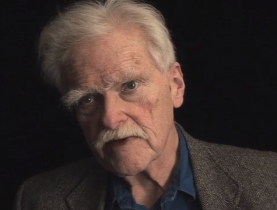
\includegraphics[width=.75\textwidth]{Bilder/movie-prev.png}}{Bilder/mouth_detection.mp4}
	\end{frame}
	\begin{frame}{Quick example}
		\centering
		\movie[width=0.5\textwidth,poster,autostart,showcontrols,loop]{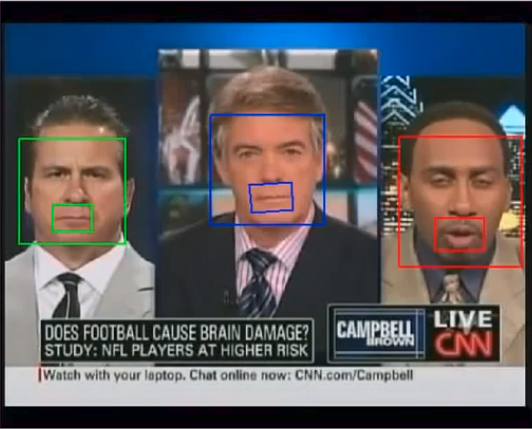
\includegraphics[width=.5\textwidth]{Bilder/movie2-prev.png}}{Bilder/speaker_detection.mp4}
		
		Interesting demo: https://www.youtube.com/watch?v=5aogzAUPilE
		
		Also interesting: https://github.com/astorfi/lip-reading-deeplearning (using audio \& visual information)
	\end{frame}
	
	
	\section{Hardware}%%%%%%%%%%%%%%%%%%%%%%%%%%%%%%%%%%%%%%%%%%%%%%%%%%%%%%%%%%%%%%%%%%%%%%%%%%%%%%%%%%%%%%%%
	
	\begin{frame}{Microphones}
		\begin{figure}[ht]
			\centering
			\subfloat[dynamic microphone]{
				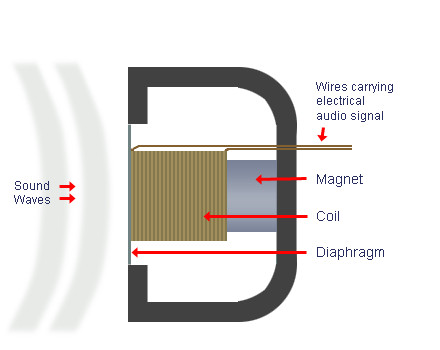
\includegraphics[width=.5\textwidth]{Bilder/mic-dynamic.jpg}
			}
			\subfloat[condenser microphone]{
				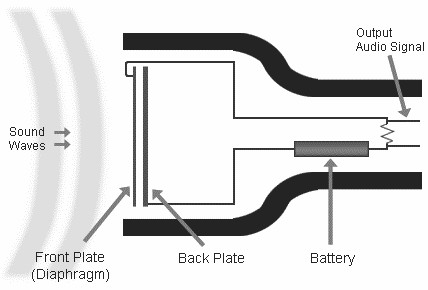
\includegraphics[width=.5\textwidth]{Bilder/Condenser-Mic-Diagram.jpg}
			}
			\caption{Different kinds of microphones. Source: http://www.onlinetuner.co}
		\end{figure}
	\end{frame}
	
	\begin{frame}{Audio}
		
		\begin{alertblock}{Microphones provide audio defined by:}
			\begin{itemize}[leftmargin=*,labelindent=50pt]
				\item[rate:] resolution in time domain
				\item[bitrate:] resolution in quality domain
				\item[endian:] representation of signal
				\item[channel:] amount of channels 
				\item[interleaving:] representation of signal by channel
			\end{itemize}
		\end{alertblock}
	\end{frame}
	
	\begin{frame}{Microphones: Polar Patterns}
		\begin{figure}[ht]
			\centering
			\subfloat[cardioid pattern]{
				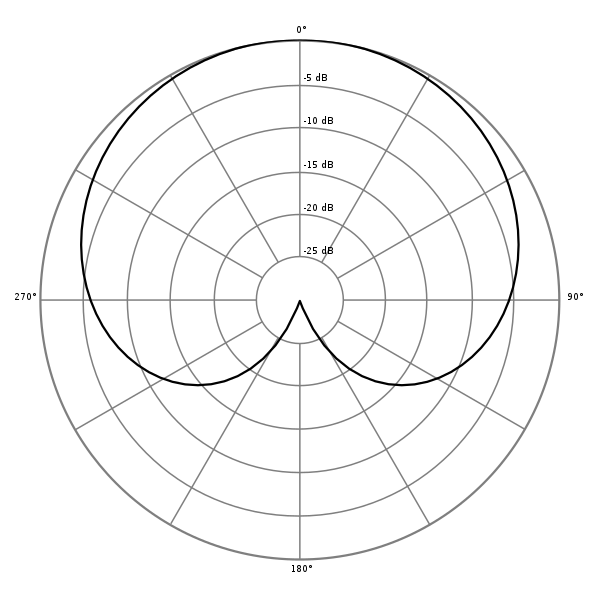
\includegraphics[width=.33\textwidth]{Bilder/Polar_pattern_cardioid.png}
			}
			\subfloat[directional pattern]{
				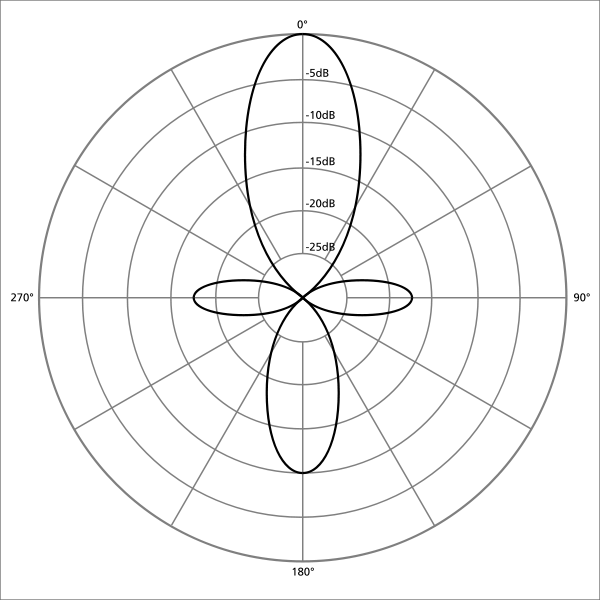
\includegraphics[width=.33\textwidth]{Bilder/Polar_pattern_directional.png}
			}
			\subfloat[omnidirectional pattern]{
				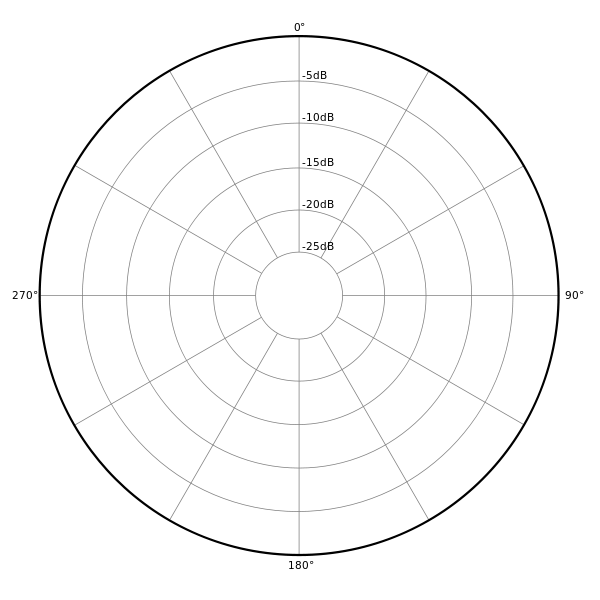
\includegraphics[width=.33\textwidth]{Bilder/Polar_pattern_omnidirectional.png}
			}
			\caption{Diffrent kinds of microphone pattern. Source: Wikipedia}
		\end{figure}
	\end{frame}
	
	\begin{frame}{Microphone Arrays}
		\begin{alertblock}{Why?}
			\begin{itemize}
				\item[-] more sensors are always better
				\item[-] several microphones can be linked together to reduce noise
				\item[-] by analysing the distribution of signals and frequencies in time we can even detect the direction from where a sound was emitted
			\end{itemize}
		\end{alertblock}
	\end{frame}
	
	\begin{frame}{Microphone Arrays II}
		\begin{figure}[ht]
			\centering
			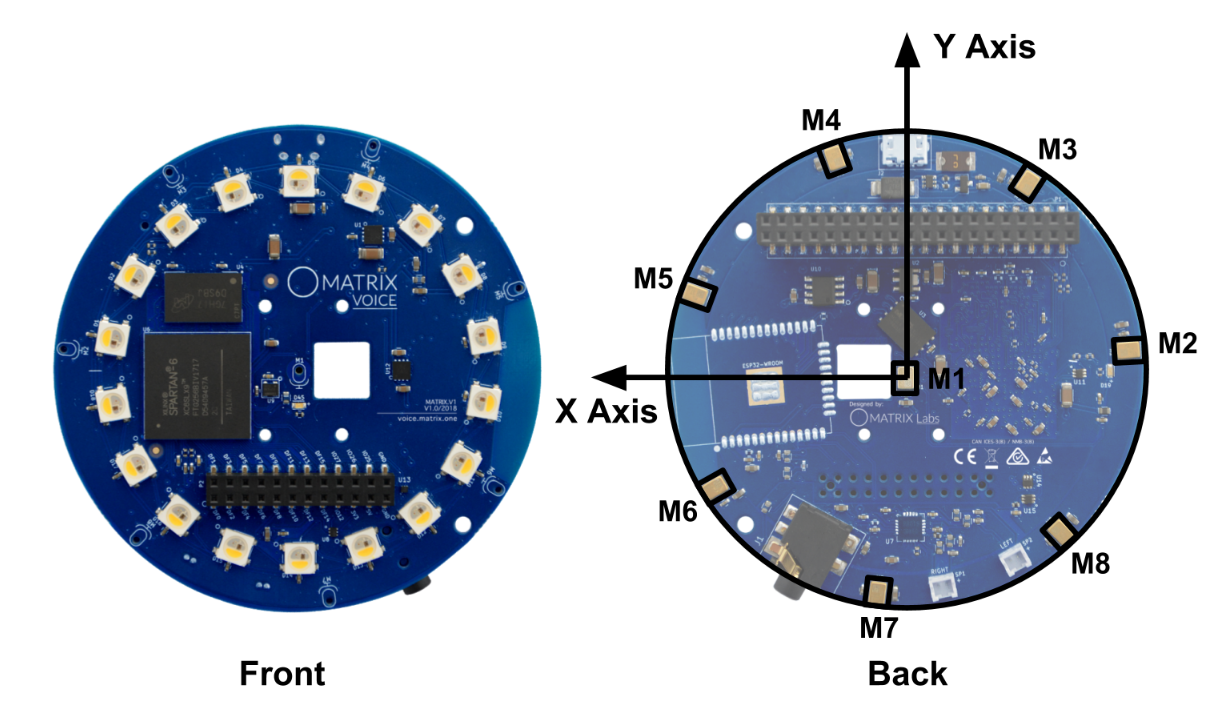
\includegraphics[width=.8\linewidth]{Bilder/mic_voice_position.png}
			\caption{Matrix Voice, a microphone array. Source: https://matrix-io.github.io/matrix-documentation/matrix-voice/resources/microphone/}
		\end{figure}
	\end{frame}
	
	\begin{frame}{What do we use?}

		\begin{alertblock}{Tobi:}
			\pause
			One or two directional microphones, 2 additional for sound source localization.
		\end{alertblock}
		
		\begin{alertblock}{Pepper:}
			\pause
			An array of four omnidirectional microphones inside of the head.
		\end{alertblock}
		
		\begin{alertblock}{Tiago:}
			\pause
			Stereo microphones in the torso (black spots under his head).
		\end{alertblock}
	\end{frame}
	
	\begin{frame}{Alsa}
		\begin{alertblock}{The Advanced Linux Sound Architecture manages all your physical and virtual microphones and speakers.}
			\begin{itemize}
				\item[-] It controls volume and gain
				\item[-] It controls rate and bitrate of captured audio, as well as other properties
				\item[-] Extensive configuration makes basically any imaginable microphone constellation possible
			\end{itemize}
		\end{alertblock}
		
		\pause
		
		\begin{alertblock}{Honorable mention: pulseaudio}
			\pause
			\begin{itemize}
				\item[-] \emph{many} extensions (called modules) to suit all kinds of needs
				\item[-] eg. virtual devices over network, on the fly filtering, etc.
			\end{itemize}
		\end{alertblock}
	\end{frame}
	
	\section{Localisation}%%%%%%%%%%%%%%%%%%%%%%%%%%%%%%%%%%%%%%%%%%%%%%%%%%%%%%%%%%%%%%%%%%%%%%%%%%%%%%%%%%%%%%%%
	
	\begin{frame}{Sound Source Localisation}
		\begin{alertblock}{Basic Idea:}
			\begin{itemize}
				\item[-] more than one microphone is required
				\item[-] four microphones are required for "exact" localisation
				\item[-] can be seperated into 2 sub-problems: time delay estimation and position estimation
				\item[-] time delay estimation guesses the time differences with which a sound arrives at different microphones
				\item[-] position estimation  tries to locate the soundsource based on these guesses
			\end{itemize}
		\end{alertblock}
	\end{frame}
	
	\begin{frame}{Time Delay Estimation}
		\begin{alertblock}{Approaches:}
			\begin{itemize}[leftmargin=*,labelindent=16pt]
				\item[-] time domain approximation
				\item[-] frequency based
				\item[-] statistical approaches
			\end{itemize}
		\end{alertblock}
		
		\begin{figure}[ht]
			\centering
			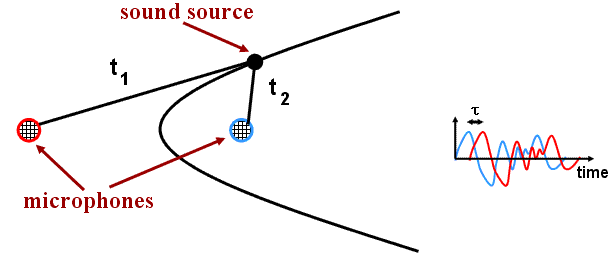
\includegraphics[width=.8\linewidth]{Bilder/ssl.png}
			\caption{Different signal run time based on distance. Source: https://cecas.clemson.edu/~stb/research/acousticloc/}
		\end{figure}
	\end{frame}
	
	\begin{frame}{Position estimation}
		\begin{alertblock}{Sound source localisation is not exact!}
			\begin{itemize}
				\item[-] TDE is just an estimation (duh)
				\item[-] because of superposition TDE may provide false positives
				\item[-] position estimation can be interpreted as (n-1)-dimensional optimization problem
				\item[-] optimization problems can be solved by eg. gradient descent or conjugate gradients
			\end{itemize}
		\end{alertblock}
		(see Mario Botsch's Scientific Computing course for more information about solving these problems)
	\end{frame}
	
	\section{Signal Enhancing}%%%%%%%%%%%%%%%%%%%%%%%%%%%%%%%%%%%%%%%%%%%%%%%%%%%%%%%%%%%%%%%%%%%%%%%%%%%%%%%%%%%%%%%%
	
	\begin{frame}{Beamforming}
		\begin{alertblock}{Basically SSL$^{-1}$}
		
			Signals of several microphones are summed up, timeshifted according to an angle of interest
		\end{alertblock}
		\begin{figure}[ht]
			\centering
			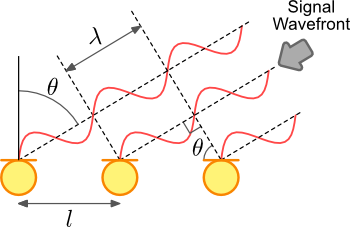
\includegraphics[width=.6\linewidth]{Bilder/beamform.png}
			\caption{Beamforming using several Receivers. Source: http://www.labbookpages.co.uk/audio/beamforming/delaySum.html}
		\end{figure}
	\end{frame}
	
	\section{Voice Activation Detection}%%%%%%%%%%%%%%%%%%%%%%%%%%%%%%%%%%%%%%%%%%%%%%%%%%%%%%%%%%%%%%%%%%%%%%%%%%%%%%%%%%%%%%%% rather done
	
	\begin{frame}{What we use}
		\begin{figure}[ht]
			\centering
			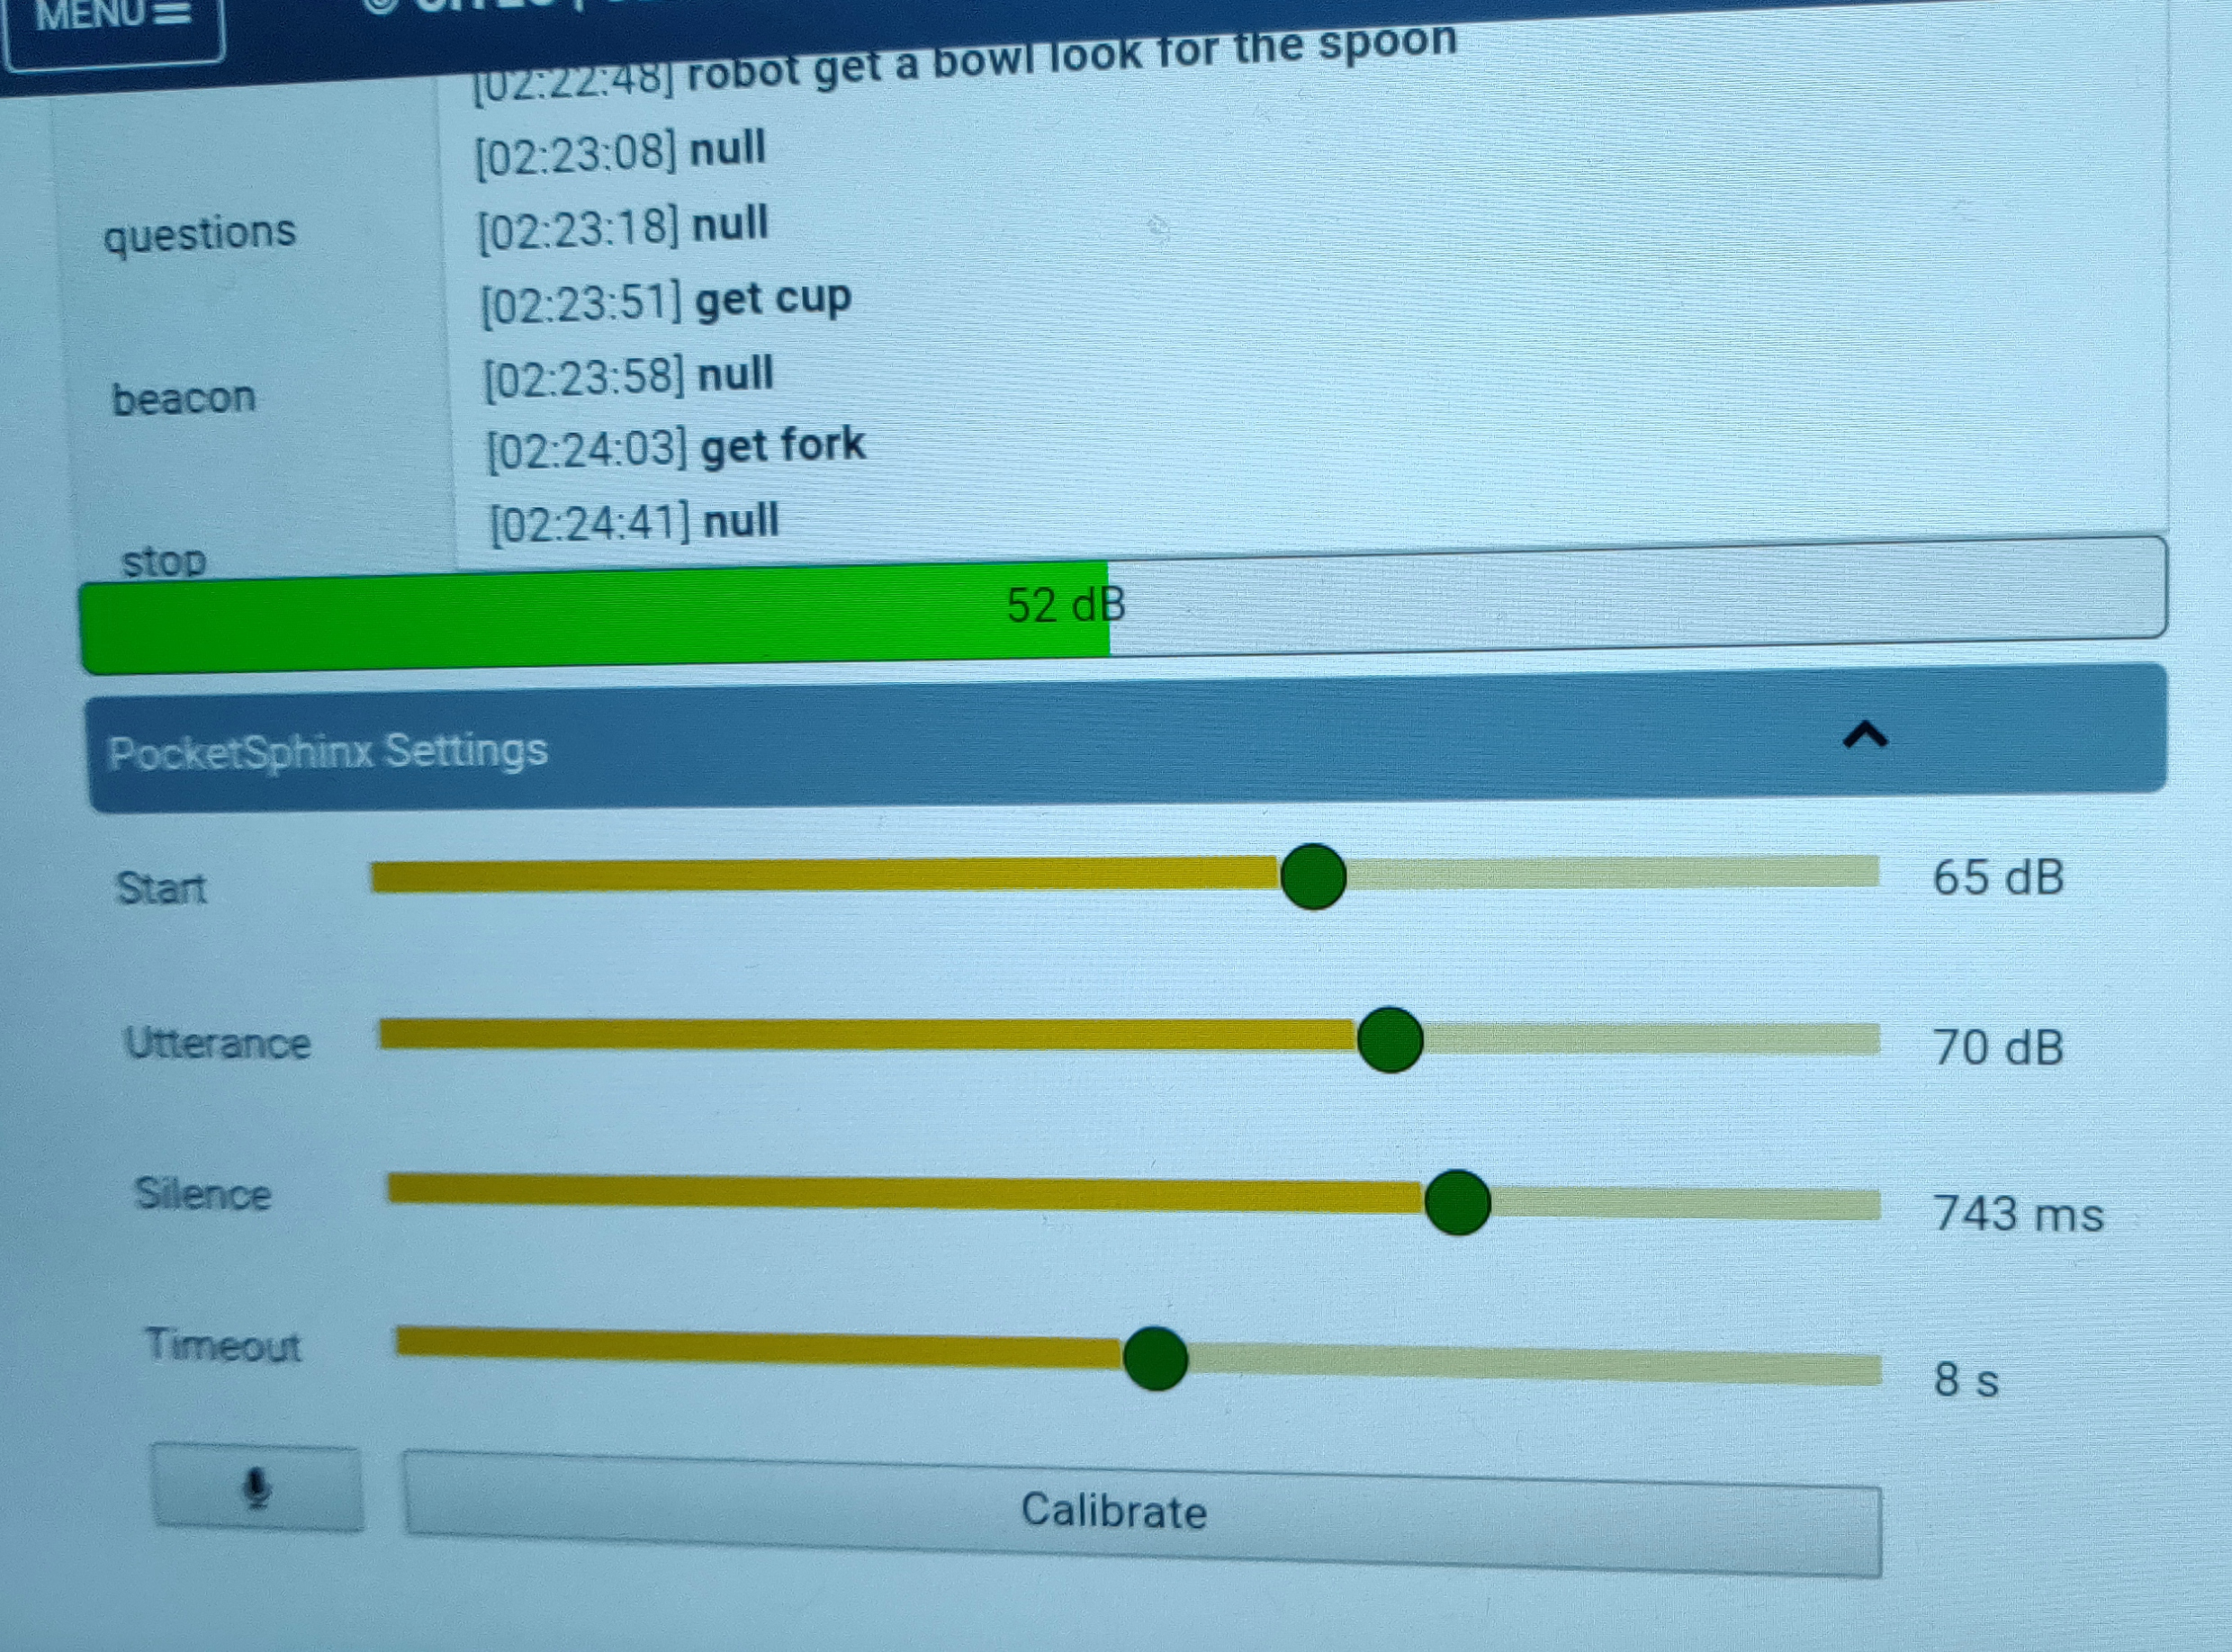
\includegraphics[width=.8\linewidth]{Bilder/VAD.jpg}
			\caption{Double threshold voice activation detection}
		\end{figure}
	\end{frame}
	
	\begin{frame}{What we use II}
		\begin{alertblock}{A voice activation detection based on audio loudness with three states: }
			\begin{itemize}[leftmargin=*,labelindent=32pt]
				\item[idle] Start in this state
				\item[starting] switch to this state if the audio $>$ StartDb and stay here as long as audio $>$ UtteranceDb
				\item[ending] switch to this state if the audio $<$ UtteranceDb and stay as long as specified via Silence, then return to idle
			\end{itemize}
			A maximum audio length can be specified via Timeout
		\end{alertblock}
	\end{frame}
	
	\begin{frame}{Other approaches}
		\begin{alertblock}{Based on...}
			\begin{itemize}[leftmargin=*,labelindent=32pt]
				\item[loudness] based on decibel calculation, it will only take into account the single most extreme value in an audio frame
				\item[energy] in contrast to loudness-based approaches, energy calculation will take all values in an audio frame into consideration
				\item[frequency] will calculate frequencies and search for those typically used by human speech
			\end{itemize}
		\end{alertblock}
	\end{frame}
	
	\section{Speaker Recognition}%%%%%%%%%%%%%%%%%%%%%%%%%%%%%%%%%%%%%%%%%%%%%%%%%%%%%%%%%%%%%%%%%%%%%%%%%%%%%%%%%%%%%%%%
	
	\section{Speech Recognition}%%%%%%%%%%%%%%%%%%%%%%%%%%%%%%%%%%%%%%%%%%%%%%%%%%%%%%%%%%%%%%%%%%%%%%%%%%%%%%%%%%%%%%%%
	
	\begin{frame}{Approaches}
		\begin{alertblock}{There are three big approaches for consumer/ robotics speech recognition:}
			\begin{itemize}
				\item[-] Hidden Markov Models
				\item[-] Deep Learing
				\item[-] Online Services
			\end{itemize}
		\end{alertblock}
	\end{frame}
	
	\begin{frame}{Hidden Markov Models}
		\begin{alertblock}{Hidden Markov models are statistical models where a system is assumed to be a markov process with hidden states.}
			\begin{itemize}
				\item[-] imagine a statemachine where the transitions are modeled by probabilities
				\item[-] states in this statemachine can be roughly understood as phonemes
				\item[-] a most probable path through the model can be computed for a given sequence of signals or data 
				\item[-] this path is can then be mapped to a spoken word or sequence of words
				\item[-] states are unknown (hidden) and assumed via probabilities
			\end{itemize}
		\end{alertblock}
	\end{frame}
	
	\begin{frame}{Sphinx}
		\begin{alertblock}{A HMM based group of application which use}
			\begin{itemize}
				\item[-] a speech model (models phonemes)
				\item[-] a dictionary (maps phonemes to words)
				\item[-] a language model (probabilities of word sequences)
			\end{itemize}
			
			Recent versions can provide quasi-free speech recognition.
		\end{alertblock}
	\end{frame}
	
	\begin{frame}{Deep Learning \& DeepSpeech}
		\begin{alertblock}{Deep Learning}
			\begin{itemize}
				\item[-] \emph{very} big field
				\item[-] computationally expensive concept to abstract high level information out of big chunks of data
			\end{itemize}
		\end{alertblock}
		\pause
		\begin{alertblock}{DeepSpeech}
			\begin{itemize}
				\item[-] ML architecture by Baidu
				\item[-] several implementations, e.g. by mozilla using tensorflow
				\item[-] detects free speech, but is somewhat phoneme based
				\item[-] currently one of the best architectures in regards to word error rate
			\end{itemize}
		\end{alertblock}
	\end{frame}
	
	\begin{frame}{Google/Bing/... Online Speechrec}
		\begin{alertblock}{Commercial "Cloud" services provided by companies like Google, Amazon, Microsoft, etc.}
			\begin{itemize}
				\item[-] kind of a blackbox
				\item[-] need \emph{fast} internet connections
				\item[-] typically better results than local speechrec
				\item[-] not free, can be quite expensive if used extensively
			\end{itemize}
		\end{alertblock}
	\end{frame}
	
	
	\begin{frame}{Grammar vs Grammarless/Freespeech}
		\begin{alertblock}{Grammar based recognition}
			\begin{itemize}
				\item[-] by restraining accepted inputs the results can be more precise
				\item[-] mapping result to action can be very easy
				\item[-] must be supported by approach \emph{and} implementation
				\item[-] best suited for controlled environments/ use cases
			\end{itemize}
		\end{alertblock}
		\begin{alertblock}{Freespeech}
			\begin{itemize}
				\item[-] usually seen in deep learning approaches
				\item[-] any spoken word can be detected
				\item[-] go-to apporach for extremely complex use cases
			\end{itemize}
		\end{alertblock}
	\end{frame}
	
	\begin{frame}{Corrected Spelling vs Phoneme based recognition}
		\begin{alertblock}{Corrected spelling}
			\begin{itemize}
				\item[-] needs a dictionary
				\item[-] guarantees correct spelling (important for further processing)
				\item[-] makes a very robust speech recognition (esp. in combination with grammars)
			\end{itemize}
		\end{alertblock}
		\begin{alertblock}{Phoneme bases recognition}
			\begin{itemize}
				\item[-] does not need any kind of dictionary
				\item[-] adapts better to new/unique words
				\item[-] usually embraced by deep learning approaches
			\end{itemize}
		\end{alertblock}
	\end{frame}
	
	\begin{frame}{What do we use?}
		\begin{alertblock}{For everyday use:}
			\pause
			\begin{itemize}
				\item (Pocket-)Sphinx
			\end{itemize}
		\end{alertblock}
		
		\begin{alertblock}{For special cases:}
			\pause
			\begin{itemize}
				\item Google Speechrec
			\end{itemize}
		\end{alertblock}
	\end{frame}
	
	\section{Natural Language Processing}%%%%%%%%%%%%%%%%%%%%%%%%%%%%%%%%%%%%%%%%%%%%%%%%%%%%%%%%%%%%%%%%%%%%%%%%%%%%%%%%%%%%%%%% rather done
	
	\begin{frame}{Idea}
		\begin{alertblock}{Just recognizing what was said does not solve all our problems. We need to \emph{understand} what was said.}
			\pause
			\begin{itemize}
				\item[-] direct mapping?
				\pause
				\item[-] keywordspotting?
				\pause
				\item[-] how to do planning?
			\end{itemize}
		\end{alertblock}
	\end{frame}
	
	\begin{frame}{Grammar Analysis}
		\begin{alertblock}{Idea: Create the grammar tree of a sentence, thus making it easier to extract information.}
		\end{alertblock}
		
		\begin{figure}[ht]
			\centering
			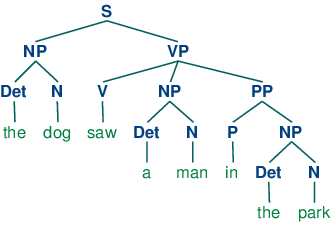
\includegraphics[width=.7\linewidth]{Bilder/grammar_tree.png}
			\caption{Example of a grammar tree. Source: https://www.nltk.org/book/ch08.html}
		\end{figure}
		
		%See also module "23-LIN-Inf Computerlinguistische Grundlagen für Informatik-Studierende"
	\end{frame}
	
	\begin{frame}{Beyong Grammar}
		\begin{alertblock}{More intensive forms of analysis can involve:}
			\begin{itemize}
				\item[-] Statistical analysis of sentences/phrases
				\item[-] tagging of phrases
				\item[-] dependency parsing
				\item[-] tokenization
			\end{itemize} 
		\end{alertblock}
	\end{frame}
	
	\begin{frame}{What do we use?}
		\begin{alertblock}{With Pocketsphinx:}
		
			\pause
			Not that much :(
		\end{alertblock}
		
		\begin{alertblock}{With Google Speechrec:}
		
			\pause
			spaCy, a python library which can...
			\begin{itemize}
				\item[-] create a grammar tree of a sentence
				\item[-] classify phrases and words (in context)
				\item[-] abstract information out of text
				\item[-] analyse the similarity of two sentences
			\end{itemize}
		\end{alertblock}
	\end{frame}
	
	\begin{frame}{spaCy example}
		\begin{alertblock}{From Wikipedia:}
		
			\emph{"RoboCup is an annual international robotics competition proposed and founded in 1996 (Pre-RoboCup) by a group of university professors (among which Hiroaki Kitano, Manuela M. Veloso, and Minoru Asada). The aim of such a competition consists of promoting robotics and AI research, by offering a publicly appealing, but formidable challenge."}
			\pause
		\end{alertblock}
		
		\begin{alertblock}{spaCy:}
			RoboCup ORG,
			1996 DATE,
			Hiroaki Kitano ORG,
			Manuela M. Veloso PERSON,
			Minoru Asada PERSON,
			AI GPE
		\end{alertblock}
	\end{frame}
	
	\begin{frame}{}
		\begin{alertblock}{Thanks for your Attention!}
		\end{alertblock}
	\end{frame}
	
	\begin{frame}{}
		\begin{alertblock}{Discussion}
		\end{alertblock}
	\end{frame}
	
\end{document}
	
	
	